\chapter{Algorithmus zur Schallquellenlokalisierung}

In diesem Kapitel werden verschiedene Ansätze zur Lokalisierung einer Schallquelle im Raum beschrieben. Die Verfahren unterscheiden sich in ihrer physikalischen Genauigkeit, im Rechenaufwand sowie in der praktischen Umsetzbarkeit. Es werden sowohl rein mathematische Interpolationsverfahren als auch modellbasierte und lernbasierte Methoden betrachtet.

\section{Grundprinzipien}

Ein präziser, aber aktuell nicht umsetzbarer Ansatz wäre die \textit{Time Difference of Arrival} (TDOA) in Kombination mit Beamforming. Dabei wird die Zeitdifferenz der Schallausbreitung zwischen mehreren Mikrofonen gemessen. Über Verfahren wie Trilateration oder GCC-PHAT lassen sich daraus Einfallswinkel und Quelle berechnen.  
Da die vorhandene Hardware jedoch keine ausreichend genaue Zeitmessung erlaubt, konnte dieser Ansatz bislang nicht praktisch umgesetzt werden.

\section{Betrachtete Verfahren}

\textbf{Bilineare Interpolation:}  
Aus den vier Eckpunkten eines Messrasters wird durch zweifache lineare Interpolation eine flache Ebene gebildet. Dies liefert eine gleichmäßige, symmetrische Heatmap, berücksichtigt jedoch keinerlei physikalische Eigenschaften der Schallausbreitung. Damit eignet sich die Methode eher zur Visualisierung als zur tatsächlichen Lokalisierung.
\begin{lstlisting}[language=JavaScript, caption={Bilineare Interpolation}]
for (let row = 0; row < 10; row++) {
  const y = row / 9;
  const rowData = [];
  for (let col = 0; col < 10; col++) {
    const x = col / 9;
    const V =
      sensorValues.d1 * (1 - x) * (1 - y) +
      sensorValues.d2 * x * (1 - y) +
      sensorValues.d3 * (1 - x) * y +
      sensorValues.d4 * x * y;
    rowData.push(Number(V.toFixed(2)));
  }
  grid.push(rowData);
}
\end{lstlisting}
\begin{minipage}[b]{0.5\textwidth}
  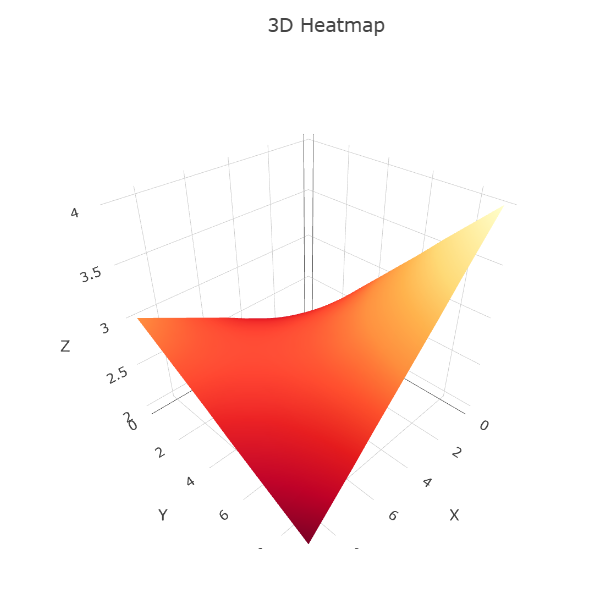
\includegraphics[width=\textwidth]{../images/Heatmap/IBHeatmap.png}
\end{minipage}

\textbf{Inverse Distance Weighting (IDW):}  
Hierbei wird der Einfluss eines Sensors umgekehrt proportional zur Distanz zur betrachteten Position gewichtet, häufig mit einem Distanzexponenten von $p=2$ (inverse quadratische Gewichtung). Das Ergebnis ist eine weiche Heatmap, deren Maximum meist in der Nähe der lautesten Sensoren liegt. Bei mehreren Schallquellen oder komplexer Raumakustik verschwimmt jedoch das Ergebnis.
\begin{lstlisting}[language=JavaScript, caption={Inverse Distance Weighting}]
const power = 2; // Distanzexponent
for (let row = 0; row < 10; row++) {
  const y = row / 9;
  const rowData = [];
  for (let col = 0; col < 10; col++) {
    const x = col / 9;
    let numerator = 0, denominator = 0;
    for (const [key, { x: sx, y: sy }] of Object.entries(sensorPositions)) {
      const value = sensorValues[key];
      const dx = x - sx;
      const dy = y - sy;
      const distance = Math.sqrt(dx * dx + dy * dy) || 0.0001;
      const weight = 1 / Math.pow(distance, power);
      numerator += value * weight;
      denominator += weight;
    }
    rowData.push(Number((numerator / denominator).toFixed(2)));
  }
  grid.push(rowData);
}
\end{lstlisting}
\begin{minipage}[b]{0.5\textwidth}
  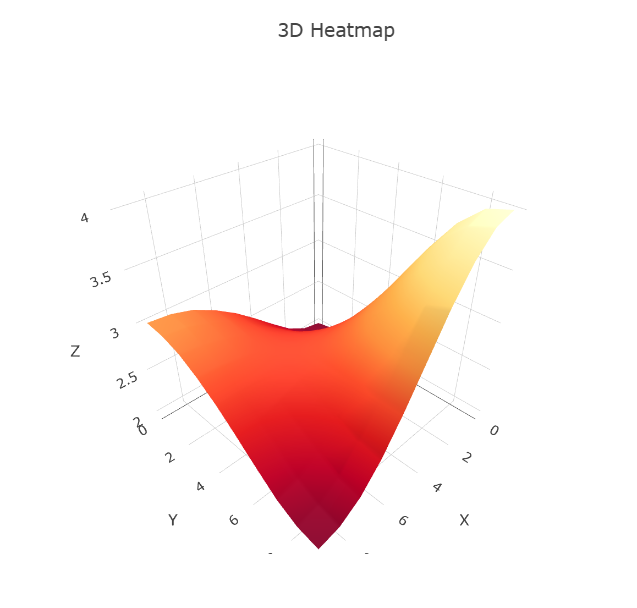
\includegraphics[width=\textwidth]{../images/Heatmap/IDWHeatmap.png}
\end{minipage}

\textbf{Physikalisches Modell – Rückwärtsprojektion:}  
Für jeden Punkt im Raum wird der erwartete Pegel an jedem Mikrofon berechnet:
\[
L = L_0 - 20 \cdot \log_{10}(d)
\]
mit $d$ als Abstand zwischen Quelle und Mikrofon. Anschließend werden die berechneten Werte mit den real gemessenen Pegeln verglichen und die Abweichungen gespeichert. Eine Heatmap zeigt die Positionen mit den geringsten Fehlern als wahrscheinlichste Quelle an.

\textbf{Maximum Likelihood Estimation (MLE):}  
Dieser statistische Ansatz modelliert die Wahrscheinlichkeit, dass eine Quelle an Position $(x, y)$ die gemessenen Pegel $s_i$ erzeugt:
\[
P = \prod_{i=1}^{n} \frac{1}{\sqrt{2\pi\sigma^2}} \cdot
\exp\left(-\frac{(s_i - (L_0 - 20\log_{10} d_i))^2}{2\sigma^2}\right)
\]
Der Punkt mit der höchsten Wahrscheinlichkeit wird als Quellenposition angenommen. Das Verfahren ist robust gegenüber Rauschen, erfordert jedoch ein präzises Modell für Messfehler.

\textbf{Weighted Centroid Localization (WCL):}  
Jeder Sensorwert wirkt wie eine „Gravitationskraft“, die die geschätzte Quelle in seine Richtung zieht. Durch Berechnung des gewichteten Mittelpunkts aller Sensoren lässt sich eine einzelne $(x,y)$-Position bestimmen, die den Schwerpunkt der Schallstärke darstellt. Gut geeignet, wenn ein dominanter Bereich im Raum deutlich lauter ist.
\begin{lstlisting}[language=JavaScript, caption={Weighted Centroid Localization (WCL)}]
	power = 2;    
  for (const [key, { x, y }] of Object.entries(sensorPositions)) {
    const value = sensorValues[key];
    const weight = Math.pow(value, power);
    weightedX += x * weight;
    weightedY += y * weight;
    weightSum += weight;
  }
\end{lstlisting}
\begin{minipage}[b]{0.5\textwidth}
  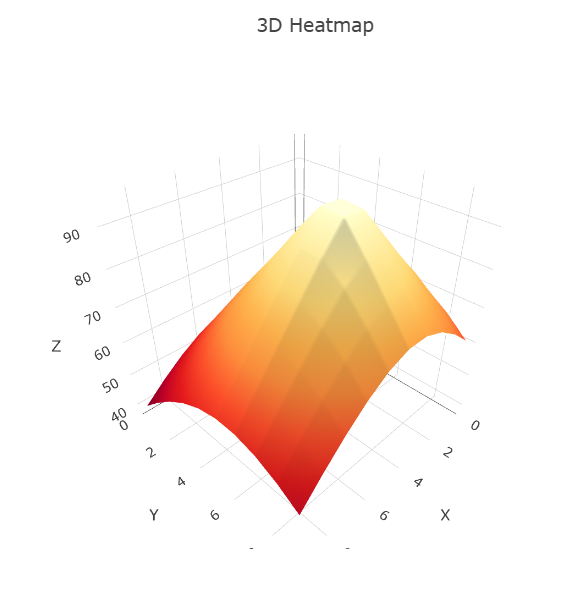
\includegraphics[width=\textwidth]{../images/Heatmap/WCLHeatmap.png}
\end{minipage}

\textbf{Machine Learning:}  
Durch Training eines Modells (z. B. KNN, Random Forest, MLP) mit bekannten Quellenpositionen und zugehörigen Pegelwerten kann die Quellenposition direkt aus den Messwerten vorhergesagt werden. Bei guter Trainingsbasis liefert dies sehr schnelle und präzise Ergebnisse. Allerdings sind umfangreiche und repräsentative Trainingsdaten erforderlich.

\textbf{Kombinierter IDW-WCL-Ansatz:}  
Zur Verbesserung der Lokalisierungsgenauigkeit wird zunächst eine IDW-Heatmap berechnet. Anschließend wird der durch WCL ermittelte Schwerpunkt durch einen zusätzlichen Peak (z. B. Gauß-Blob) verstärkt und in die Heatmap eingeblendet. Dadurch lassen sich weiche Verteilungen mit einem klaren Maximum kombinieren.
\begin{lstlisting}[language=JavaScript, caption={Kombinierter IDW-WCL-Ansatz}]
    for (let row = 0; row < gridSize; row++) {
      const y = row / (gridSize - 1);
      const rowData = [];

      for (let col = 0; col < gridSize; col++) {
        const x = col / (gridSize - 1);
        let numerator = 0;
        let denominator = 0;

        for (const point of interpolationPoints) {
          const dx = x - point.x;
          const dy = y - point.y;
          const distance = Math.sqrt(dx * dx + dy * dy) || epsilon;
          const weight = 1 / Math.pow(distance, idwFlatteningPower);
          numerator += point.value * weight;
          denominator += weight;
        }

        const interpolatedValue = numerator / denominator;
        rowData.push(Number(interpolatedValue.toFixed(2)));
      }

      grid.push(rowData);
    }
\end{lstlisting}
\begin{minipage}[b]{0.5\textwidth}
  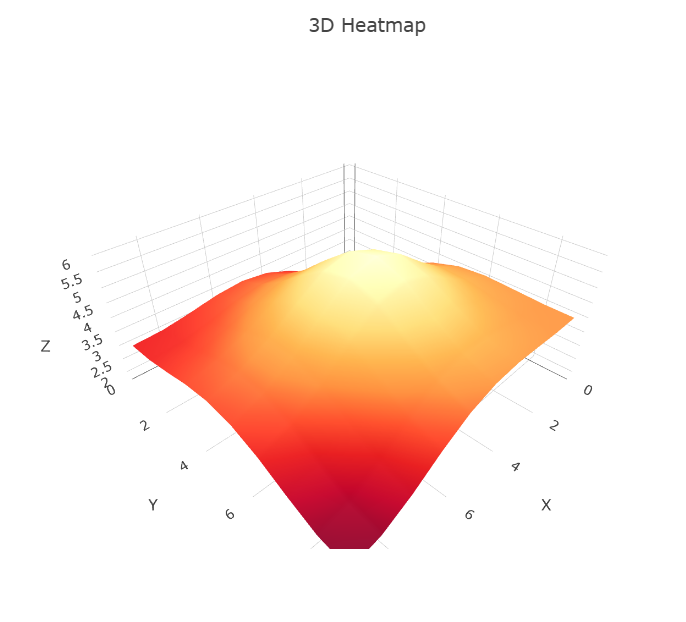
\includegraphics[width=\textwidth]{../images/Heatmap/IDWWCLHeatmap.png}
\end{minipage}

\section{Vergleich der Verfahren}

\begin{center}
\renewcommand{\arraystretch}{1.2}
\begin{adjustbox}{max width=\textwidth}
\begin{tabular}{|l|l|p{3cm}|p{3cm}|p{2.3cm}|}
\hline
\textbf{Methode} & \textbf{Typ} & \textbf{Vorteile} & \textbf{Nachteile} & \textbf{Quelle bestimmbar?} \\
\hline
Bilineare Interpolation & Interpolation & Schnell, symmetrische Heatmap & Kein physikalischer Bezug & Ungefähr \\
\hline
IDW & Interpolation & Einfach, intuitiv, glatte Heatmap & Kein klares Maximum & Ungefähr \\
\hline
Physikalisches Modell & Modellbasiert & Realitätsnah & Rechenintensiv, Annahmen nötig & Ja (Heatmap) \\
\hline
MLE & Wahrscheinlichkeit & Robust, statistisch fundiert & Modell für Fehler nötig & Ja (Wahrscheinlichkeit) \\
\hline
WCL & Schätzwert & Einfach, schneller Indikator & Ungenau bei asymmetrischen Verteilungen & Ja (Koordinate) \\
\hline
Machine Learning & Lernbasiert & Sehr schnell nach Training & Trainingsdaten nötig & Ja (xy direkt) \\
\hline
\end{tabular}
\end{adjustbox}
\end{center}

\section{Fazit}

Aus den Tests ergeben sich folgende Tendenzen:  
\begin{itemize}
    \item \textbf{Machine Learning} liefert bei guter Umsetzung die besten Ergebnisse, ist jedoch mit hohem Initialaufwand verbunden.
    \item \textbf{WCL} eignet sich gut, um den ungefähren Lautstärkenschwerpunkt im Raum zu bestimmen.
    \item \textbf{IDW} ist hilfreich, um Unterschiede in der Schallverteilung („hinten lauter als vorne“) darzustellen.
    \item \textbf{MLE} bietet hohes Potenzial für präzise Ortung, ist jedoch rechenintensiv und komplex in der Parametrisierung.
\end{itemize}

Eine Kombination aus IDW und WCL hat sich als vielversprechend erwiesen, um eine aussagekräftige Heatmap mit einem klar erkennbaren Maximum zu erzeugen.
Zudem ist diese Methode relativ einfach zu implementieren und benötigt keine aufwändige Kalibrierung.
Die Heatmap wird mit aktuellen Daten getestet, somit kann der Algorythmus durch die gewichtung von IDW und WCL angepasst werden.